\newpage
\subsection{Implementing FastCards}
\visHeader
\hypertarget{fastCard vis}{}

\begin{itemize}

\item[$\blacktriangleright$] To introduce fast cards to our learning box go to the metamodel and create the new \texttt{eclass}, \texttt{FastCard}. Quick-link
to \texttt{Card} and choose \texttt{Inheritance} from the context menu (Fig.~\ref{fig:sdm_fastcard_1}).

% INCORRECT IMAGE: missing operation printCard()
\begin{figure}[htp]
\begin{center}
  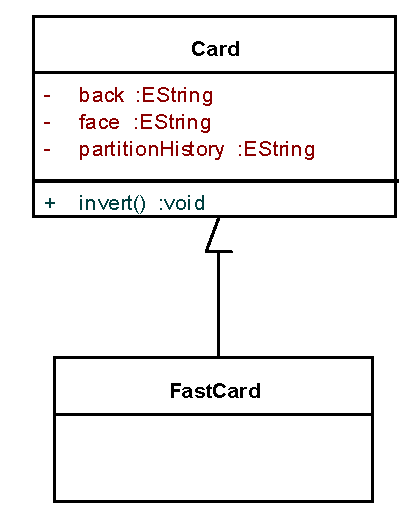
\includegraphics[width=0.4\textwidth]{fastcard}
  \caption{Fast cards are a special kind of card. {\bf UPDATE}}  
  \label{fig:sdm_fastcard_1}
\end{center}
\end{figure}

\item[$\blacktriangleright$] Now go to the SDM \texttt{check} in \texttt{Partition} and extend the control flow as depicted in Fig.~\ref{fig:sdm_fastcard_2}.
 
\item[$\blacktriangleright$] Add new story nodes \texttt{isFastCard?} and \texttt{promote FastCard} and drag and drop a bound object variable
\texttt{fastcard} \emph{of type} \texttt{FastCard} into \texttt{is fast card?}.

\begin{figure}[htbp]
\begin{center}
  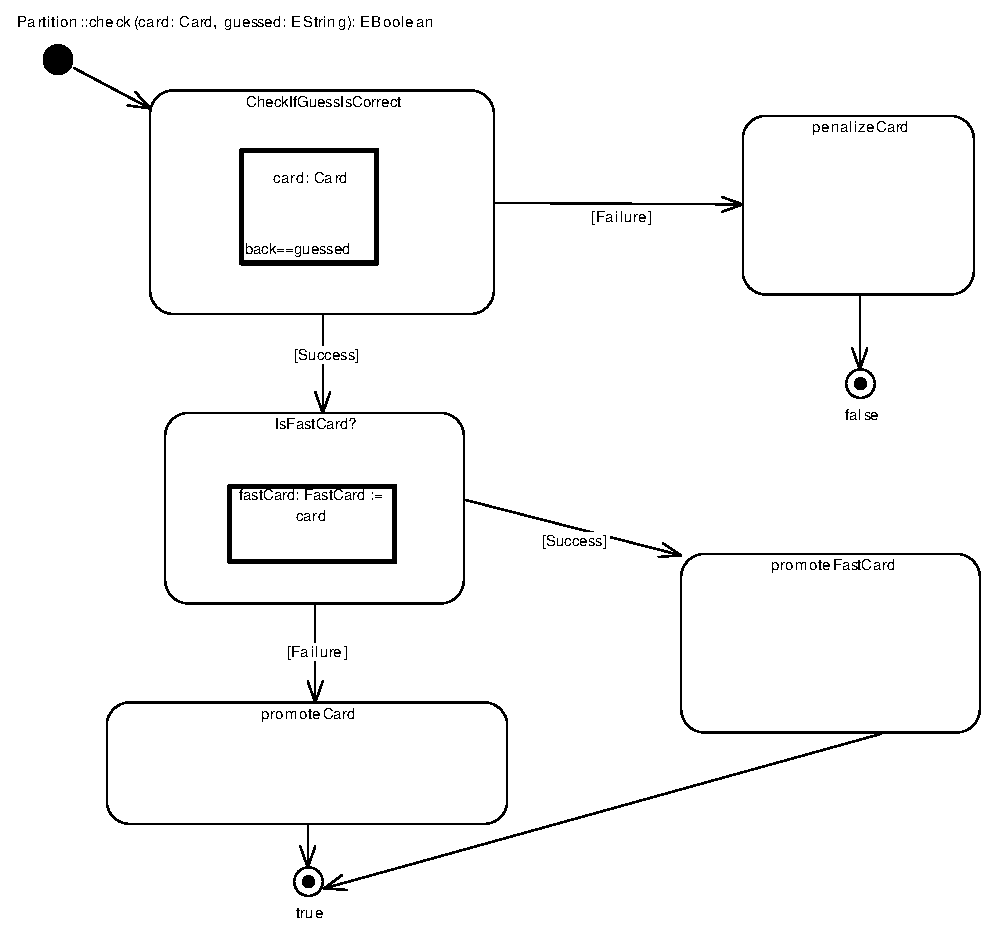
\includegraphics[width=1.2\textwidth]{fastcard_controlflow.pdf}
  \caption{Extend check to handle fast cards.}  
  \label{fig:sdm_fastcard_2}
\end{center}
\end{figure}

\end{itemize}



\begin{itemize}
  
\item[$\blacktriangleright$] To create a binding for \texttt{fastcard}, choose the \texttt{Binding} tab in the \texttt{Object Variable Properties} dialogue (Fig.~\ref{fig:sdm_fastcard_3}).

\begin{figure}[htbp]
\begin{center}
  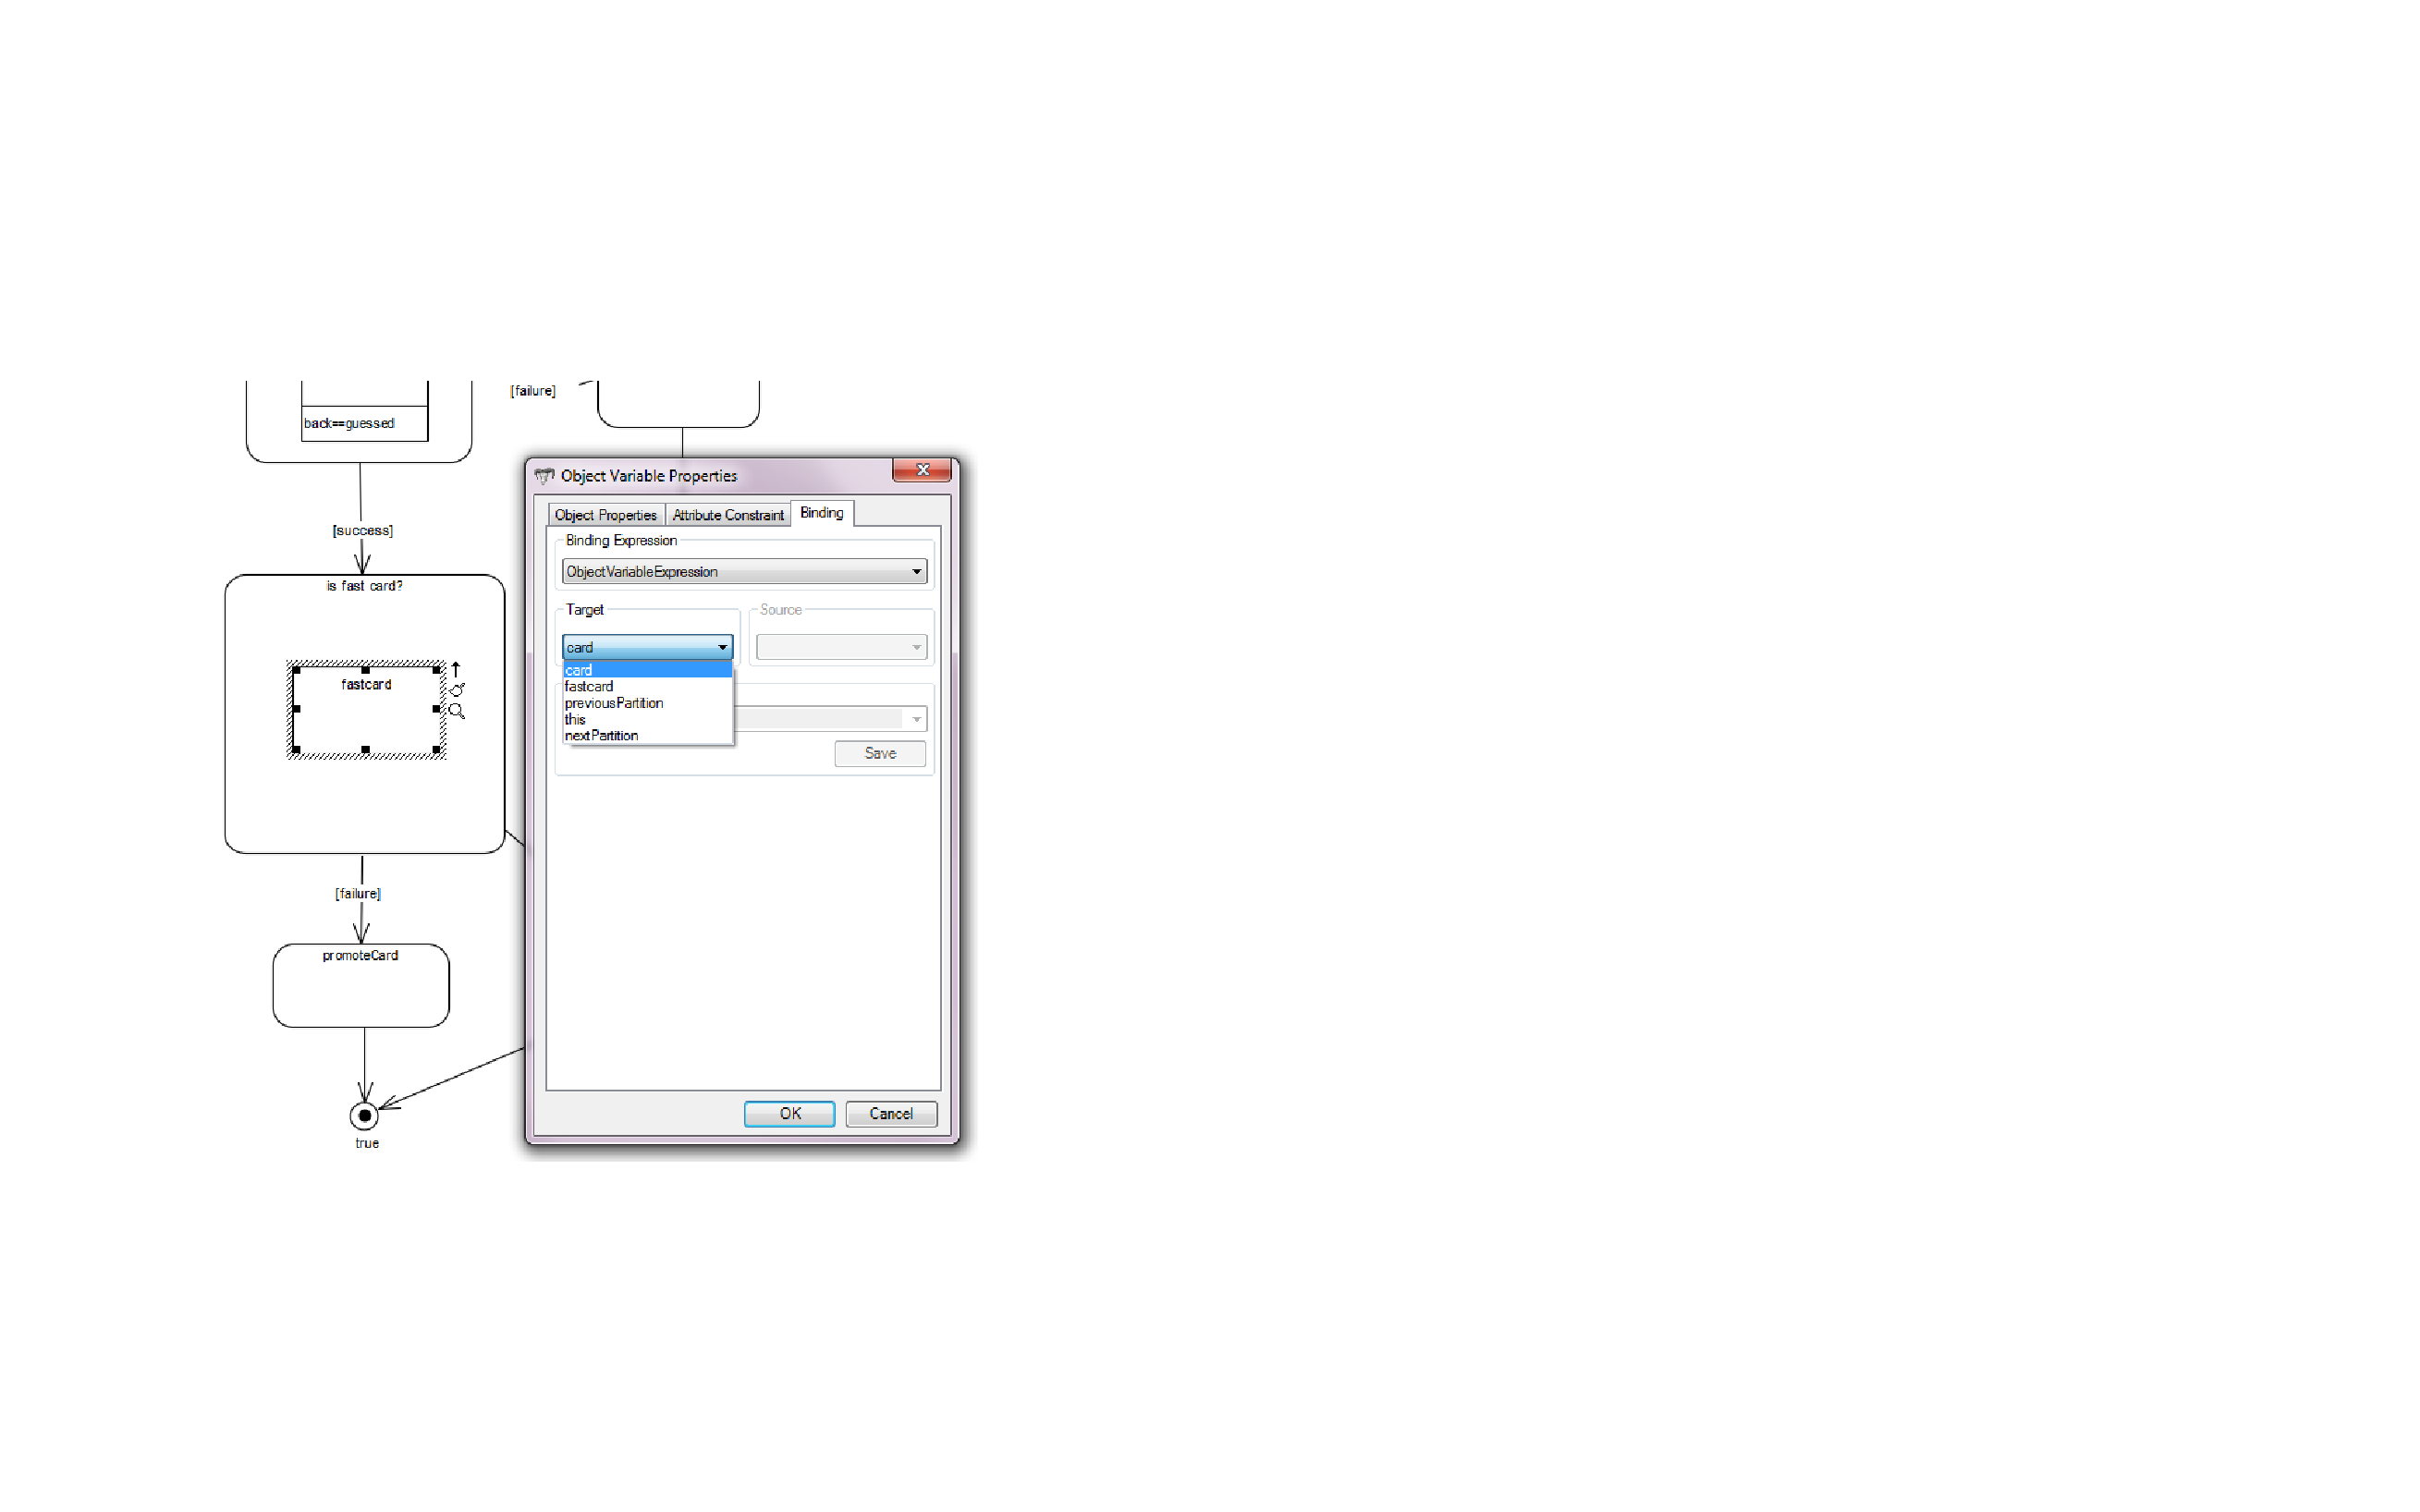
\includegraphics[width=0.5\textwidth]{fastcard_bindingexp}
  \caption{Create a binding for \texttt{fastcard}.}  
  \label{fig:sdm_fastcard_3}
\end{center}
\end{figure}

As usual, all our expression types can be used for the \texttt{Binding Expression}.  
Since we already know all the types let's consider what each type would mean in this context: 
\begin{description}
  \item[MethodCallExpression:]~\\ This would allow invoking a method and binding
  its return value to the object variable.  This is how non-primitive return
  values of methods can be used safely in SDMs.
  
  \item[ParameterExpression:]~\\ This could be used to bind the object variable
  to a parameter of the method.  If the object variable is of a different type
  than the parameter (e.g. a subtype) this represents basically a successful
  typecast if the pattern matches.
  
  \item[LiteralExpression:]~\\ As usual this can be anything and is literally
  copied with a surrounding typecast into the generated code.  Using
  LiteralExpressions too often is usually a sign for not thinking in a
  \emph{pattern oriented} manner and is considered a \emph{bad smell}.

  
  \item[ObjectVariableExpression:]~\\ This can be used to refer to other object
  variables in preceding story nodes.  Just like for ParameterExpressions, this
  represents a simple typecast if the types of the \texttt{target} and the
  object variable with the binding are different.
\end{description}

In our case, we could use a ParameterExpression or an ObjectVariableExpression as \texttt{card} is indeed a parameter \emph{and} has already been used in
\texttt{checkIfGuessIsCorrect}. 

\item[$\blacktriangleright$] Since we haven't used ObjectVariableExpressions before, lets try it out! Choose \texttt{ObjectVariableExpression} as the type of
binding expression, and \texttt{card} from the drop-down menu as the target. If you've done everything right, the binding should be visualised concisely as in
Fig.~\ref{fig:sdm_fastcard_4}.
 
\begin{figure}[htbp]
\begin{center}
  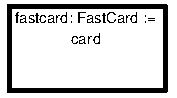
\includegraphics[width=0.2\textwidth]{visual_bindingexp}
  \caption{Visualisation for binding expression.}  
  \label{fig:sdm_fastcard_4}
\end{center}
\end{figure}

% Maybe include a footnote hyperlink to 'extract' in case user needs a reminder on how to do? (this chapter is fairly large, after all..)
\item[$\blacktriangleright$] To complete the SDM, extract the story pattern of \texttt{promote FastCard} and specify the pattern according to
Fig.~\ref{fig:sdm_fastcard_5}.
The fast card is transferred from the current partition \texttt{this}, to the last partition in the box, which is identified with an appropriate \mbox{NAC}

\begin{figure}[htbp]
\begin{center}
  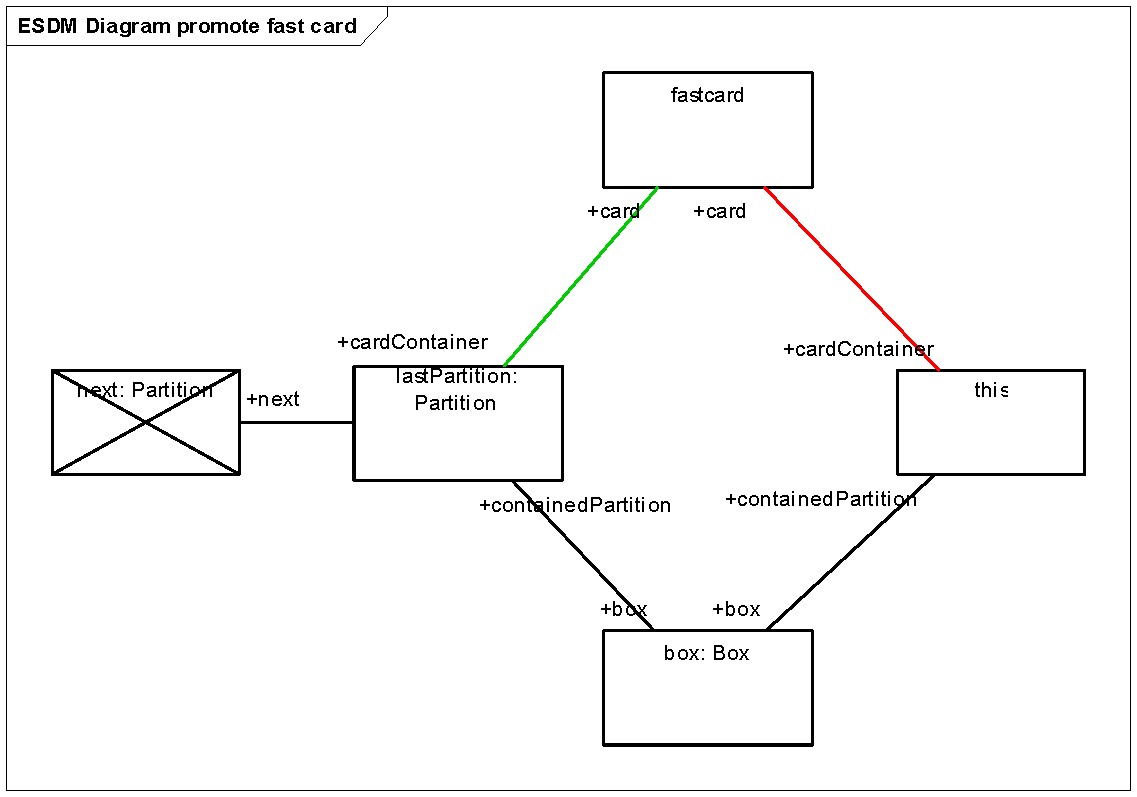
\includegraphics[width=0.9\textwidth]{promoteFastCard}
  \caption{Story pattern for handling fast cards.}  
  \label{fig:sdm_fastcard_5}
\end{center}
\end{figure}

\item[$\blacktriangleright$] Inspect Fig.~\ref{fig:promoFastCardFinal} to see how this is finalized in the you-know-what syntax.

\item[$\blacktriangleright$] You have now completed every method signature from your abstract syntax using SDMs - fantastic work! Validate, export, and generate
code for your metamodel. Inspect the implementation for \texttt{check}.  Can you find the generated type casts for \texttt{fastcard}?

\item[$\blacktriangleright$] At this point, we encourage you to read each of the textual SDM sections to understand the full scope of eMoflon's features
(which start on page~\hyperlink{page.11}{11}) but you are, of course, free to carry on
\end{itemize}
